% Files using this must be two subfolders
% deep. Adjust the number of ../ for the
% depth of the file.
% Imports
\usepackage{fancyhdr}
\usepackage{geometry}
\usepackage{icomma}
\usepackage{amsmath}
\usepackage{multicol}
\usepackage{mathptmx}
\usepackage{anyfontsize}
\usepackage{t1enc}
\usepackage{tabto}
\usepackage{listings}
\usepackage{filecontents}
\usepackage{subcaption}
\usepackage{tikz}
\usepackage[parfill]{parskip}
\usepackage{graphicx}
\usepackage[]{mdframed}
\usepackage{amsmath}
\usepackage[makeroom]{cancel}
\usepackage{pgfplots}
\usepackage{pgfplotstable}
\usepackage{xfrac}
\usepackage{amssymb}
\usepackage{mathtools}
\pgfplotsset{compat=1.18}
\usetikzlibrary{patterns}
\usepgfplotslibrary{polar}
\usepgfplotslibrary{fillbetween}

\geometry{margin=2.5cm}

\newcommand{\name}{Kaleb Burris}
\newcommand{\classname}{MATH F253, Elizabeth S. Allman, University of Alaska Fairbanks}
\newcommand{\assignment}{FILL IN ASSIGNMENT NAME}

\pagestyle{fancy}

\fancyhead[L]{
    \name 
    \newline
    \classname
    \newline
    \assignment
}

\newcommand{\horizontal}{\noindent\rule{\hsize}{0.4pt}}

\setlength{\headheight}{42pt}
\setlength{\headsep}{0.25in}
\setlength{\columnsep}{0.35cm}
\setlength{\columnseprule}{1pt}

\usepackage[T1]{fontenc}
\usepackage{lmodern}

\usepackage{graphicx}
\graphicspath{ {./lab0images/} }

% Put class number, class name, and professor 
% name.
% Use only in case of emergency, this
% should be covered by the preamble.
% \renewcommand\classname{}

% Put the assignment name with \S if 
% necessary for the section and the question 
% numbers.
\renewcommand\assignment{Lab 0: Introduction to Physics, 1/24/2023, Partner: }

\begin{document}

    % Templates
    \iffalse
    % Use these for equations.
    \begin{equation*}
        \begin{gathered}
            Equations go here.
        \end{gathered}
    \end{equation*}

    % Use this if a line of math is too long.
    \resizebox{\hsize}{!}{$Long equation goes here$}

    % Use these for multiple columns.
    \begin{multicol*}{# of columns}
        % Remove the * if you want the columns to be balanced.
    \end{multicol*}

    % Use this to add a horizontal line.
    \horizontal

    \fi

    % Begin homework here.
    %%%%%%%%%%%%%%%%%%%%%%

    \section*{Lab 01: Introduction to Physics}

    \subsection*{Apparatus}

    \begin{itemize}
        \item Position and Velocity Graphs
        \begin{itemize}
            \item foam board
            \item motion detector
            \item lab quest
            \item meter stick
        \end{itemize}
        \item Jumping Students
        \begin{itemize}
            \item Force plates
            \item lab quest
            \item board
        \end{itemize}
    \end{itemize}

    \subsection*{Objective}

    The purpose of this lab is to introduce you to some of the concepts you will learn in physics this semester, without using equations. You’ll take some measurements and make some plots, but mostly you will be observing and thinking about what you see while trying to make sense of it. 

    \subsection*{Theory}

    To understand the world around us we make observations while looking for patterns and generalizations. From this we try to determine cause-and-effect relationships and make predictions. These days “making observations” frequently refers to using a search engine, but do not worry, kinesthetic-tactile learning is still a thing. One of the great benefits of a lab class is simply handling the equipment! 


    \subsection*{Procedure} 
    
    Instructions are bullet-points, questions to be answered are numbered, information such as this is just text. Note: “graph” and “plot” are used interchangeably.

    \pagebreak

    \section*{(Station 1) Position / Time and Velocity / Time Graphs}

    \begin{center}
        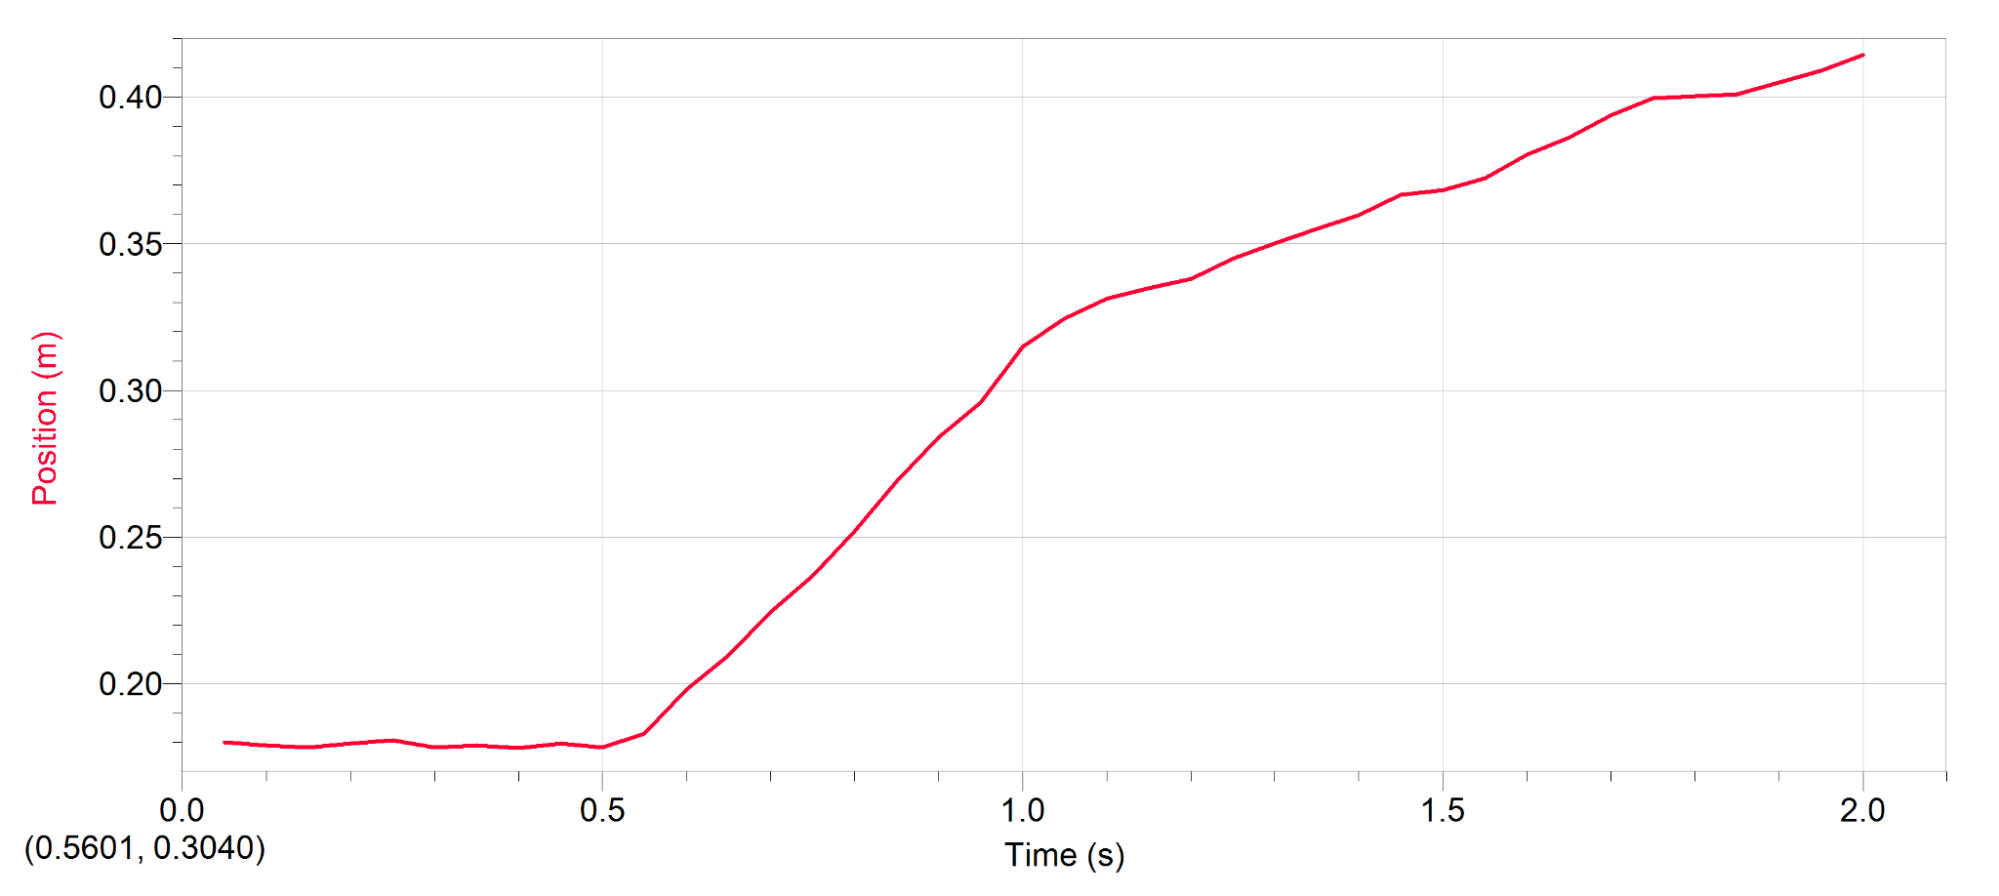
\includegraphics[width=\textwidth]{image9.png}

        Constant speed with a sudden flat slow down.

        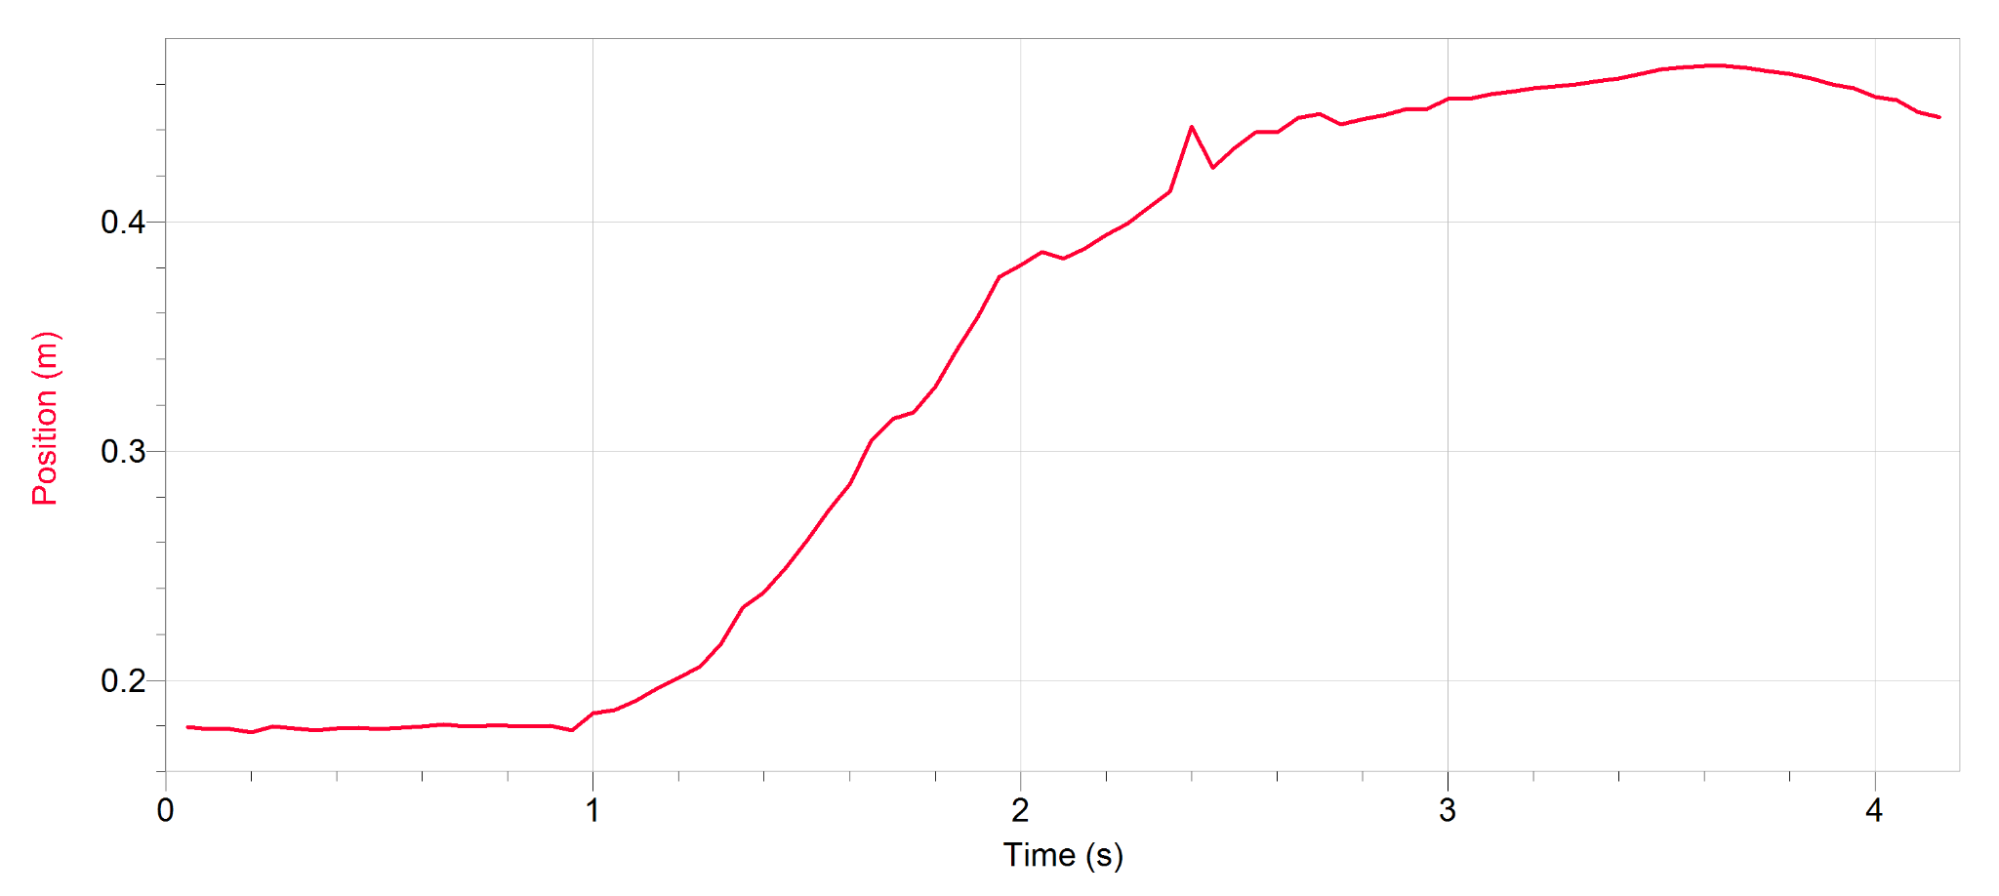
\includegraphics[width=\textwidth]{image10.png}
        
        The object speeds up and then slows down to a stop.

        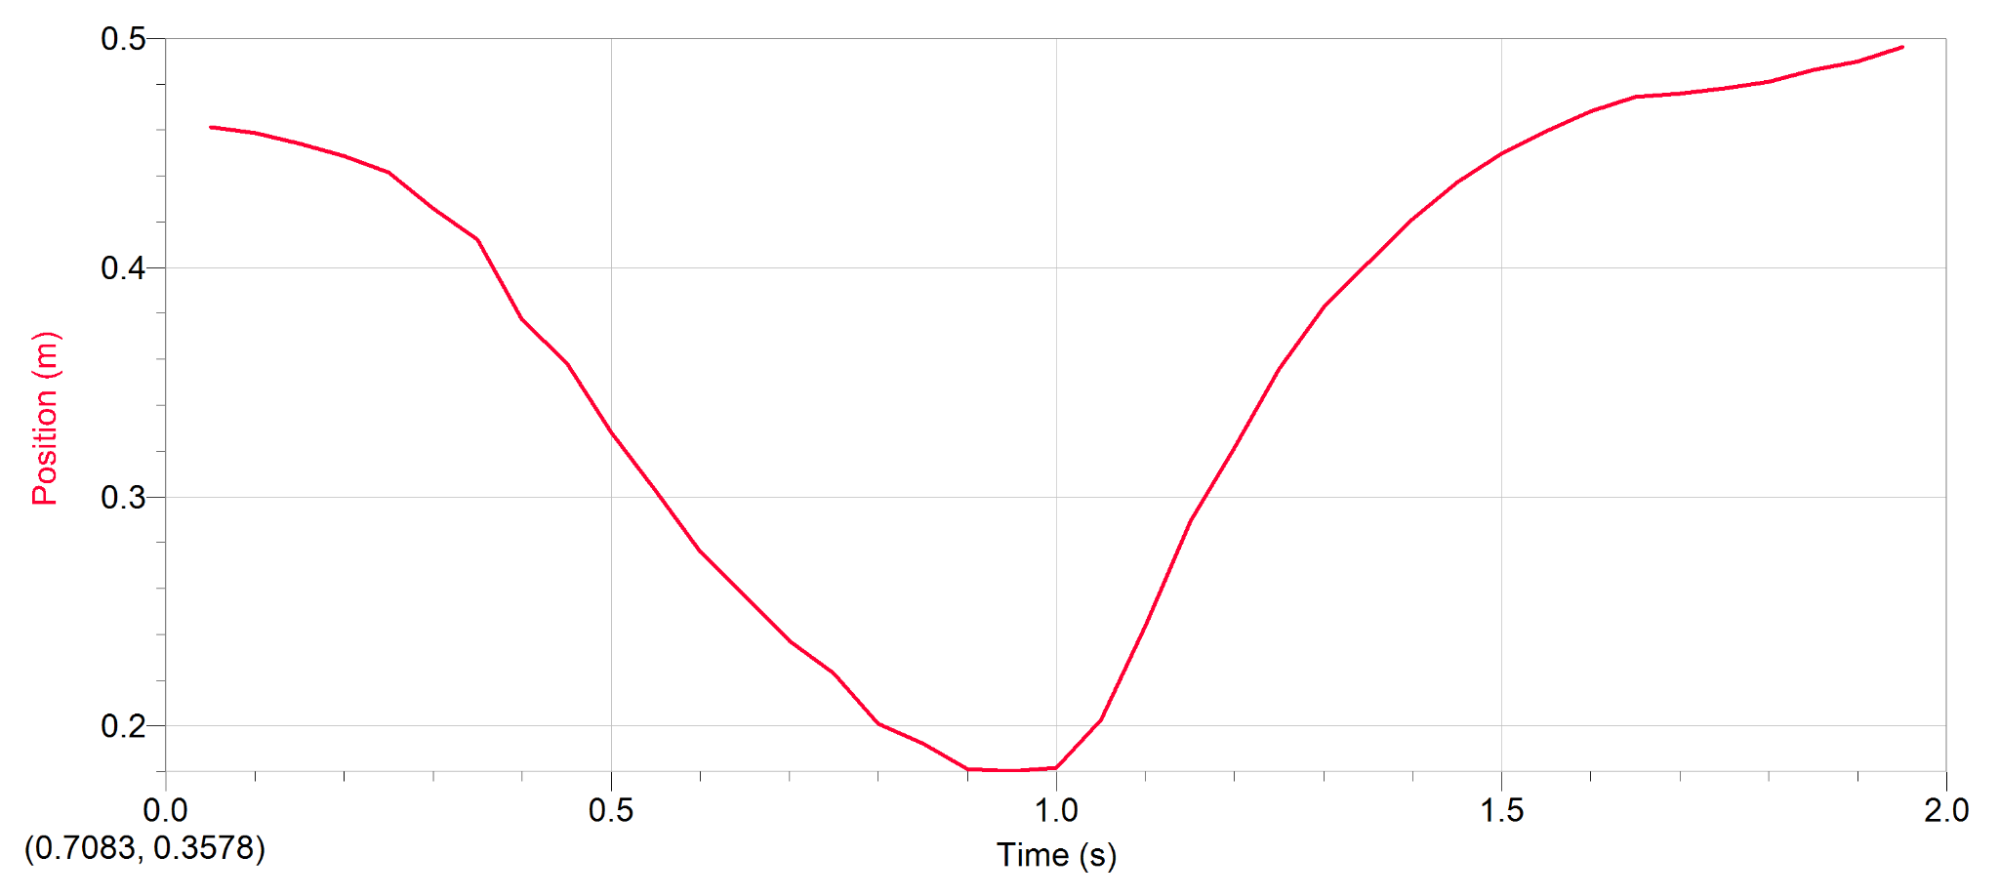
\includegraphics[width=\textwidth]{image1.png}
        
        A constant speed that suddenly flips and the object travels at the same speed in the direction it came from.

        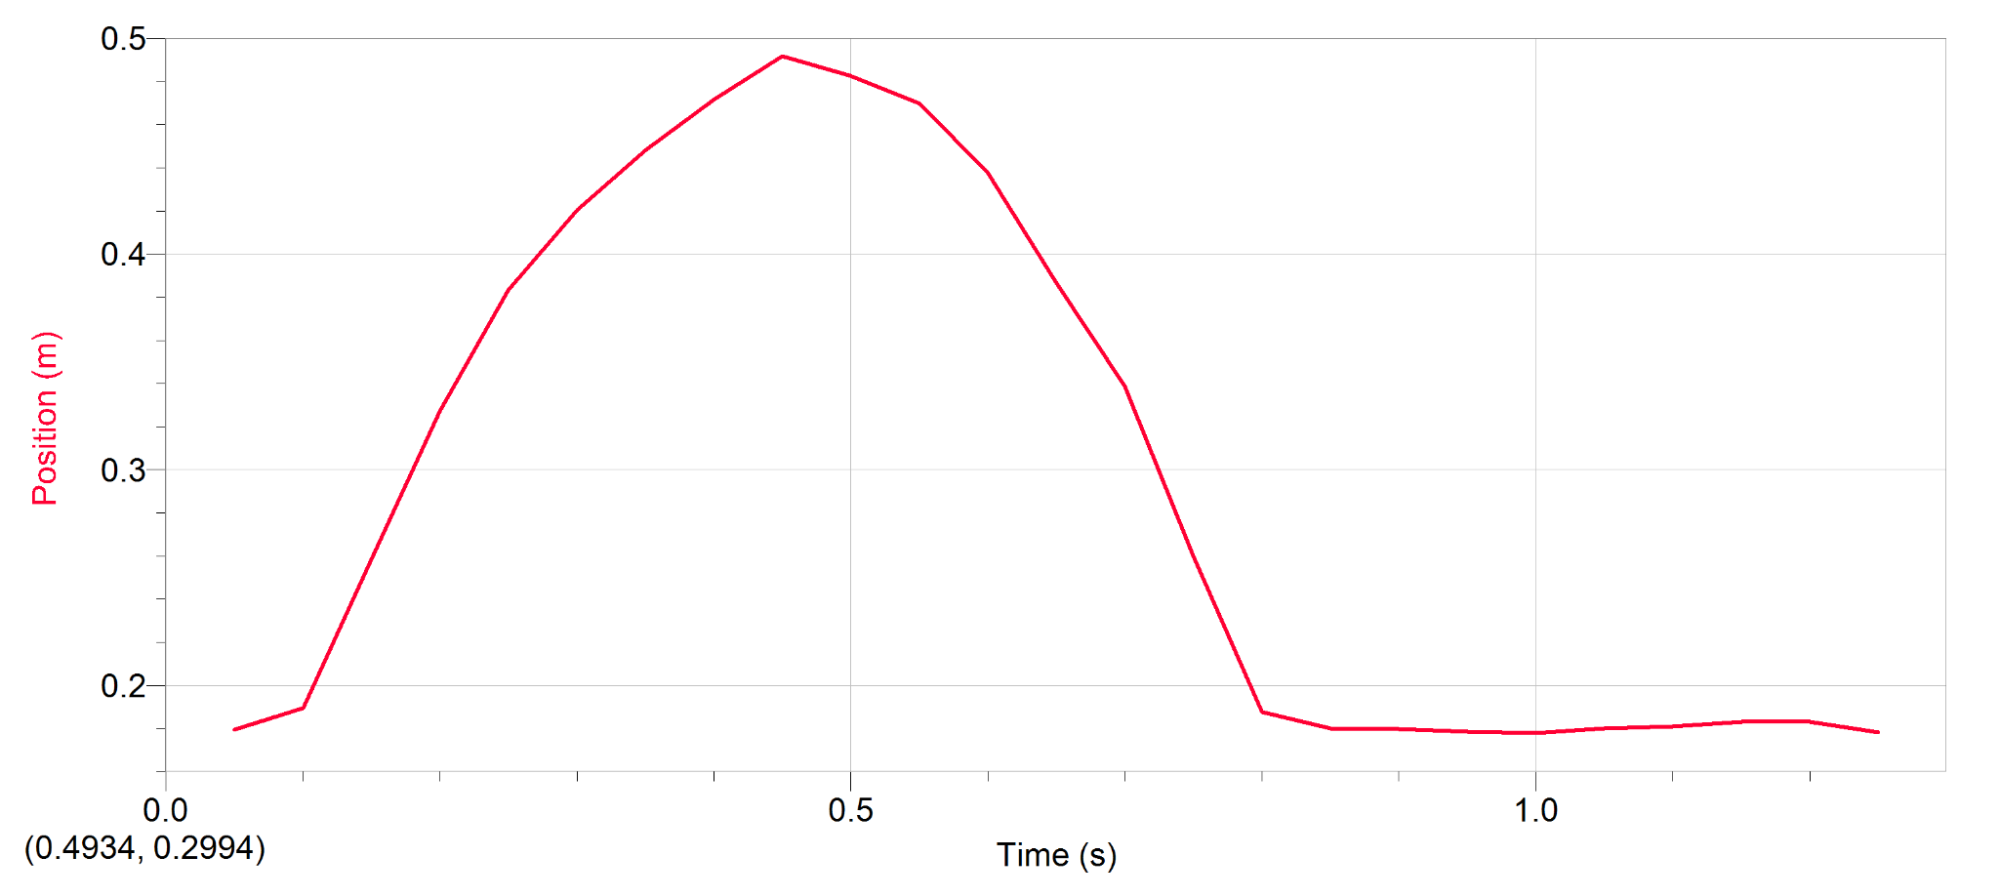
\includegraphics[width=\textwidth]{image8.png}
        
        The object starts moving quickly, slows to a stop and then speeds up back toward the sensor.

        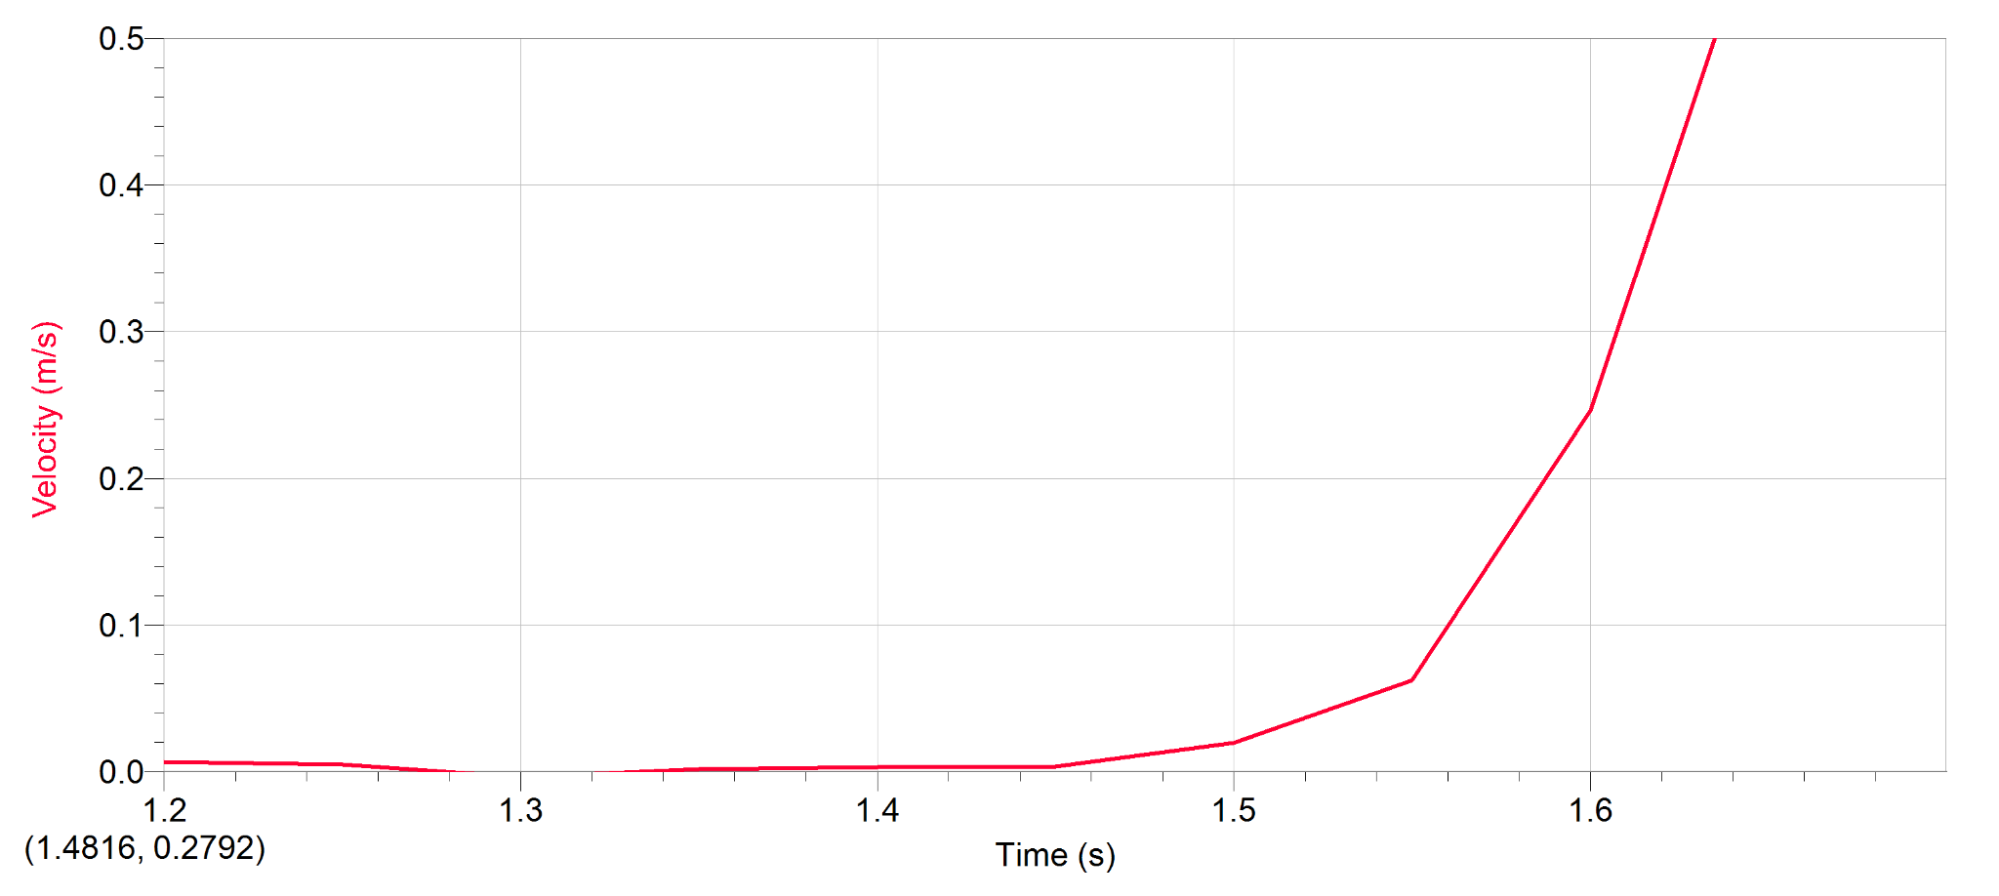
\includegraphics[width=\textwidth]{image7.png}
        
        The object is still and then slowly speeds up as it travels away.

        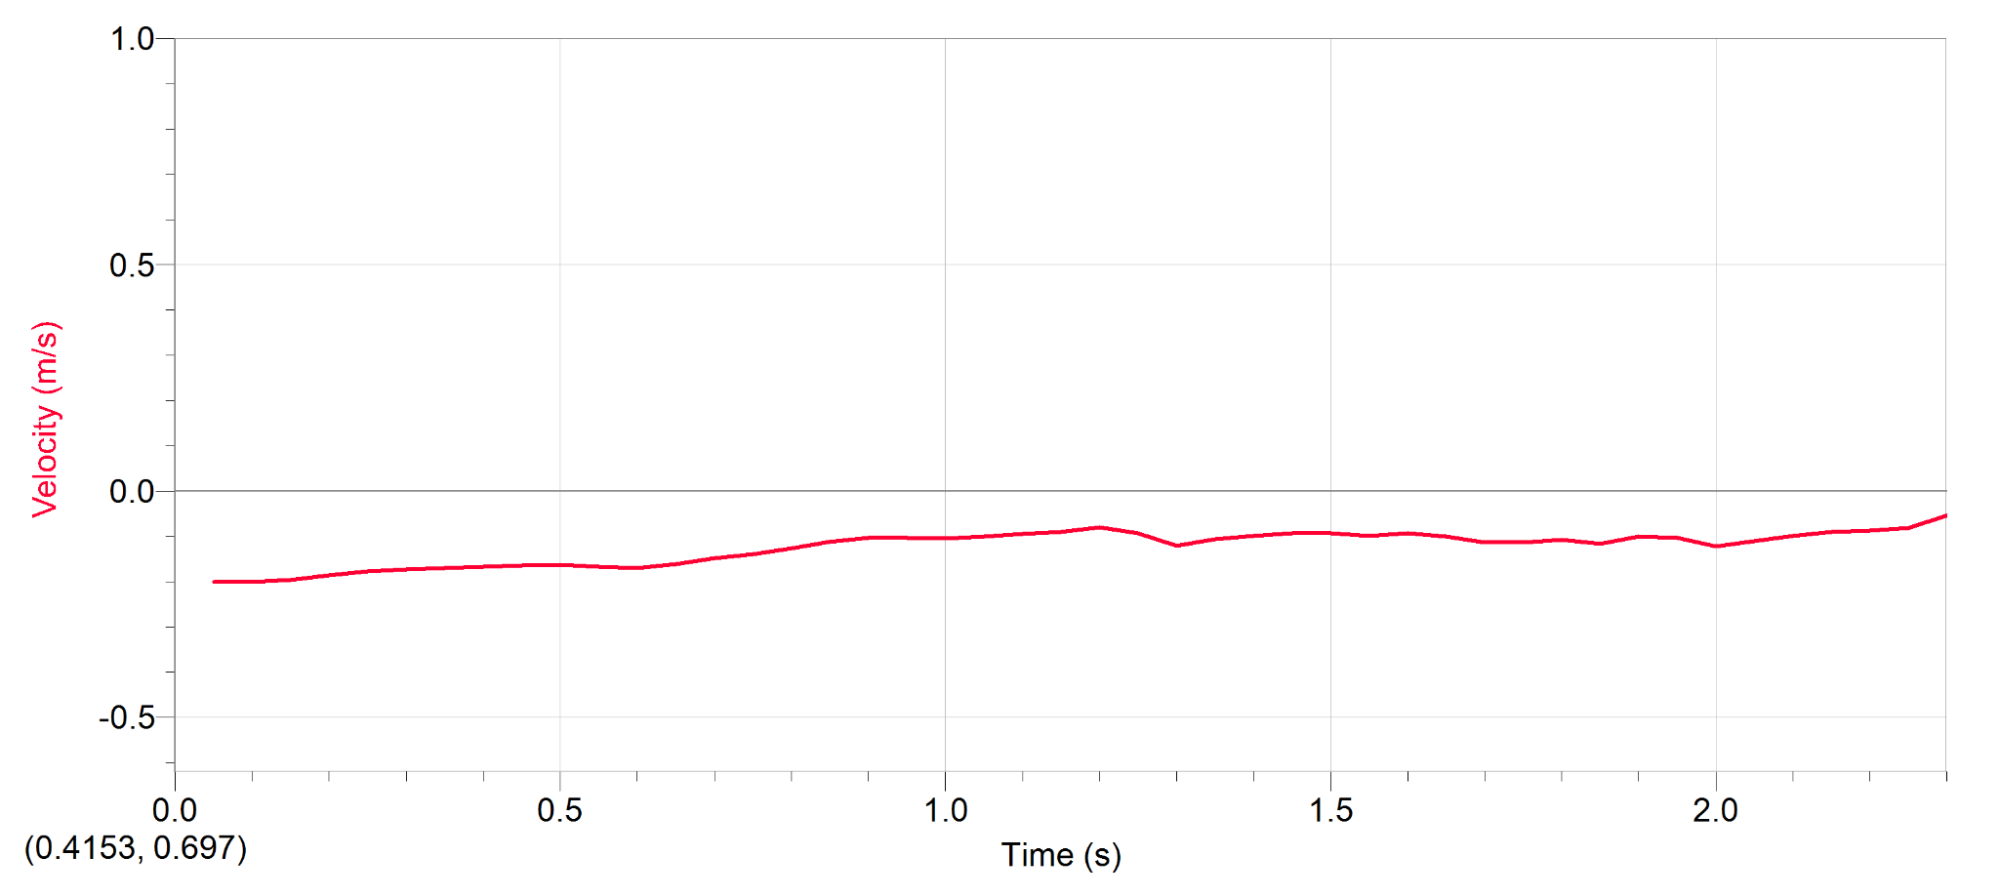
\includegraphics[width=\textwidth]{image18.png}
        
        The object travels away at a steady rate.

        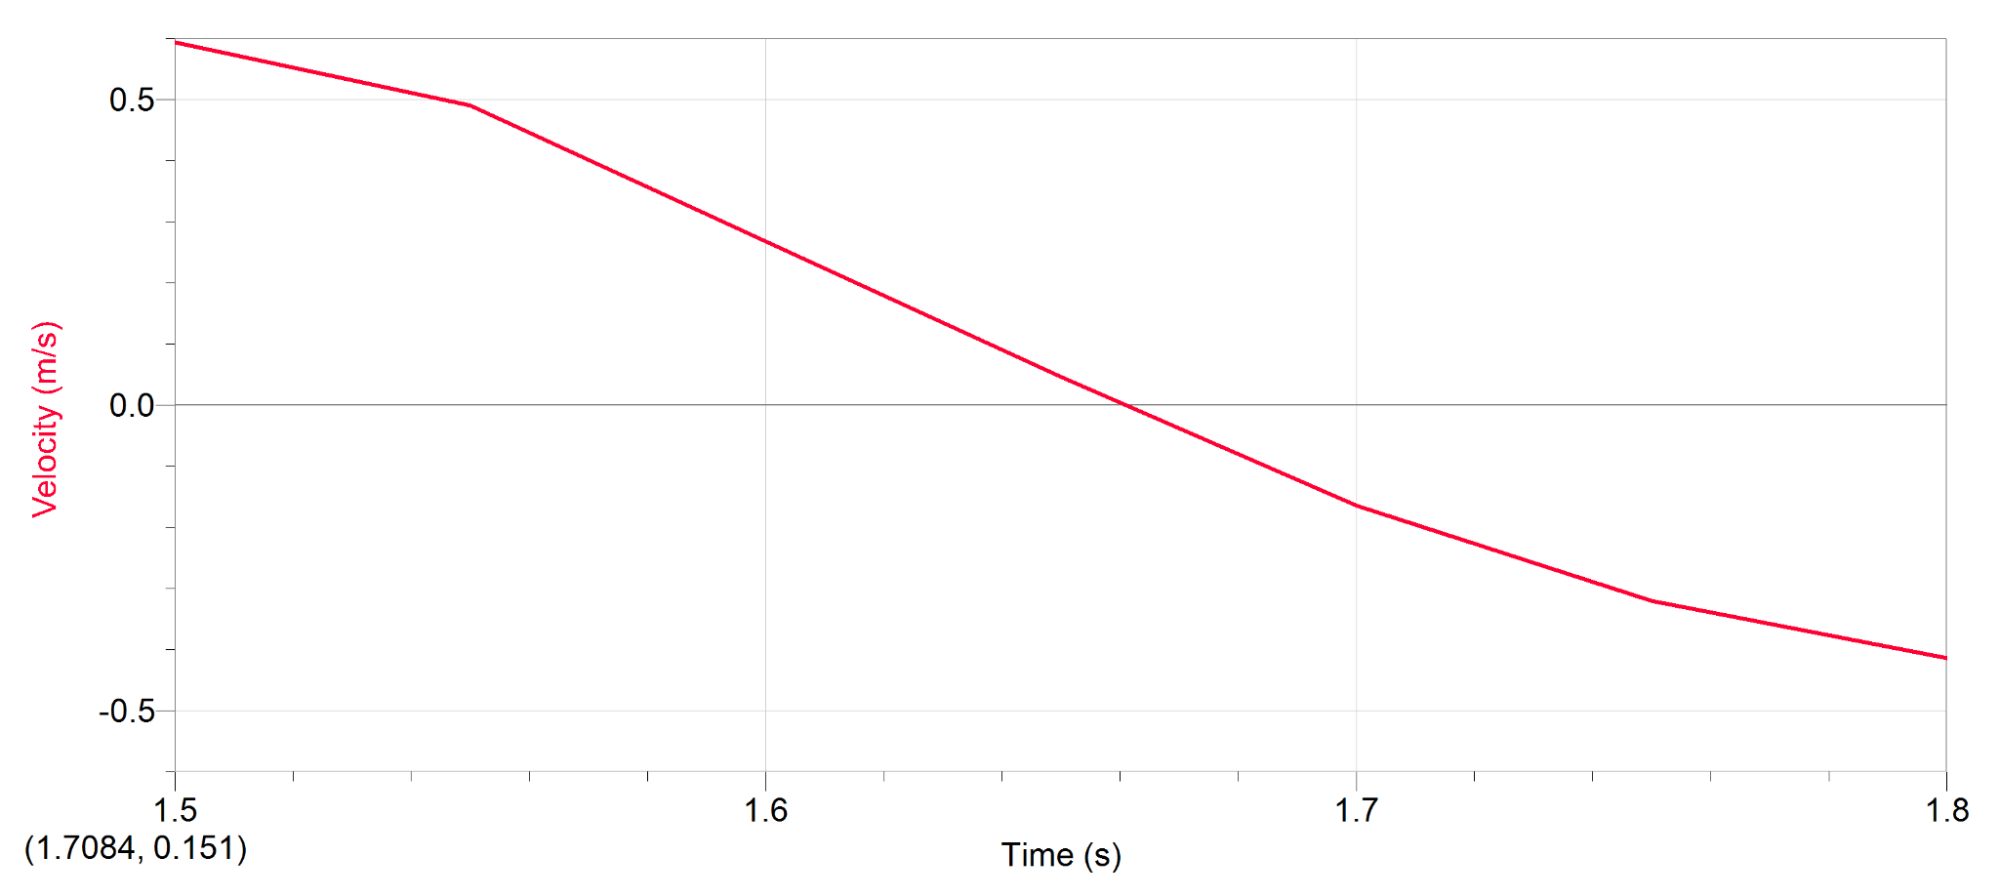
\includegraphics[width=\textwidth]{image4.png}
        
        The object starts moving quickly, slows to a stop, and reverses direction and begins accelerating backwards.
    \end{center}

    Follow up questions:

    \paragraph*{1.} How can you determine velocity information from a position / time graph? Be specific.

    \begin{mdframed}
        However steep the position graph is, is how large the velocity vector is. A steep downward direction of the position graph indicates the object is accelerating quickly in the negative direction and vice versa.
    \end{mdframed}

    \paragraph*{2.} When a position / time graph has a curved (not straight) line, what can you say about your motion?
    
    \begin{mdframed}
        The motion is either accelerating or decelerating, the velocity is changing as time goes on.
    \end{mdframed}
    
    \paragraph*{3.} When a velocity / time graph crosses the time axis, what can you say about your motion?

    \begin{mdframed}
        The motion has swapped directions; it goes from coming towards the sensor to going away or from going away to coming towards the sensor.
    \end{mdframed}

    \pagebreak

    \section*{(Station 2) Jumping Students}
        \paragraph*{1.}

        \begin{mdframed}
            The graph will jump to a set value and remain relatively smooth.

            \begin{tikzpicture}
                \begin{axis}[
                    ymin=0,
                    ymax=30000000,
                    xmin=0,
                    xmax=5,
                    xlabel=Seconds(s),
                    ylabel=Newtons(n)
                ]
                    \addplot[]{20000000};
                \end{axis}
            \end{tikzpicture}
        \end{mdframed}

        \paragraph*{2.}

        \begin{mdframed}
            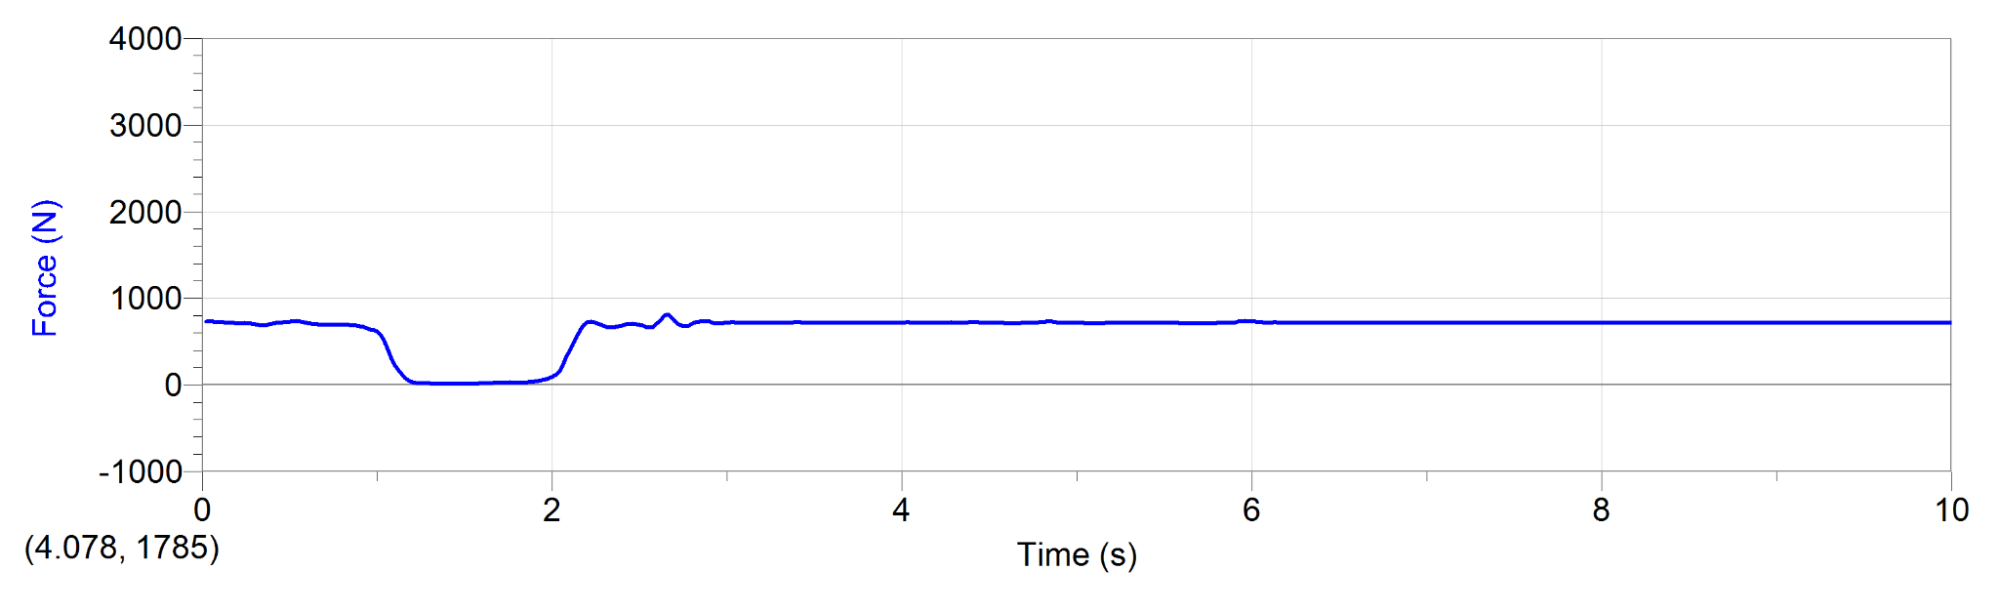
\includegraphics[width=\textwidth]{image3.png}

            $\uparrow$ This is my partner's graph.

            When stood still on the plate, the graph remained flat, with some up/down sections as I got on/off.
        \end{mdframed}

        \paragraph*{3.}

        \begin{mdframed}
            1180N
        \end{mdframed}

        \paragraph*{4.}

        \begin{mdframed}
            It will be a series of sharp spikes up/down as I bounce on it.
        \end{mdframed}

        \paragraph*{5.}

        \begin{mdframed}
            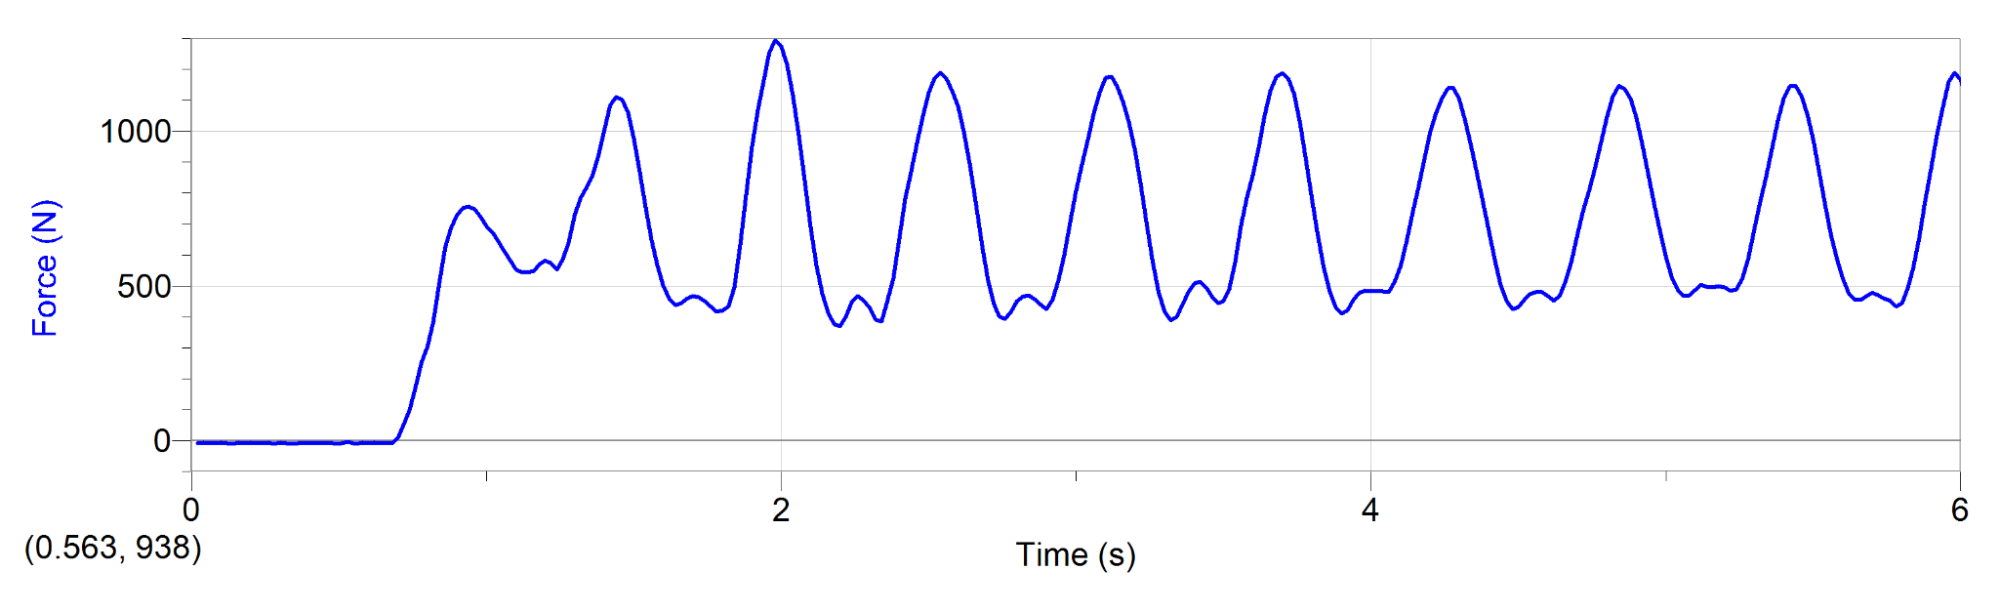
\includegraphics[width=\textwidth]{image2.png}

            While flapping my arms, the graph was sinusoidal with a slight ``hickup''/``heartbeat''.
        \end{mdframed}

        \paragraph*{6.}

        \begin{mdframed}
            The weight will shoot up very high, and then rocket down to my usual weight.
        \end{mdframed}

        \paragraph*{7.}

        \begin{mdframed}
            Small: 1786N

            Medium: 2024N

            Large: 2487N
        \end{mdframed}

        \paragraph*{8.}

        \begin{mdframed}
            Small: 0.17s

            Medium: 0.26s

            Large: 0.4s
        \end{mdframed}

        \paragraph*{9.}

        \begin{mdframed}
            The peak on landing was slightly higher, but the time spend accelerating was longer than the time it took to decelerate.
        \end{mdframed}

        \paragraph*{10.}

        \begin{mdframed}
            The ground is less elastic than human flesh.
        \end{mdframed}

        \paragraph*{11.}

        \begin{mdframed}
            The force should be the same or extremely close for either sensor.
        \end{mdframed}

        \paragraph*{12.}

        \begin{mdframed}
            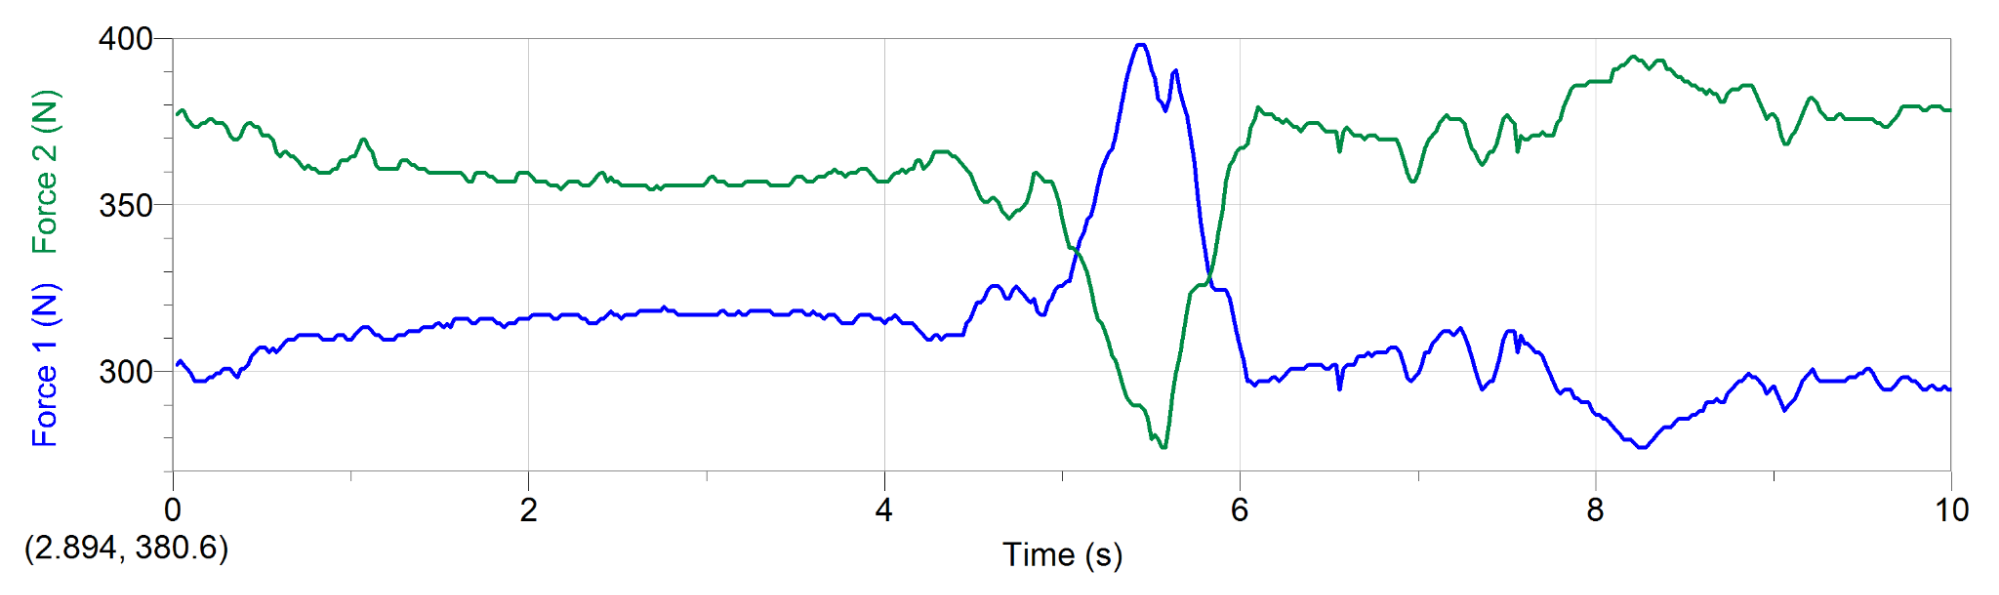
\includegraphics[width=\textwidth]{image17.png}

            Force Plate 1: ~ 320 N
            
            Force Plate 2: ~ 360 N
        \end{mdframed}

        \paragraph*{13.}

        \begin{mdframed}
            One sensor will start high and the other low, and the values will intersect and invert with each other.
        \end{mdframed}

        \paragraph*{14.}

        \begin{mdframed}
            Not recorded.
        \end{mdframed}

        \paragraph*{15.}

        \begin{mdframed}
            I think the force plot will be parabolic as it goes from my weight to a low value, back to my weight.
        \end{mdframed}

        \paragraph*{16.}
    
        \begin{mdframed}
            The force increased rather linearly as I went from one side to the other.

            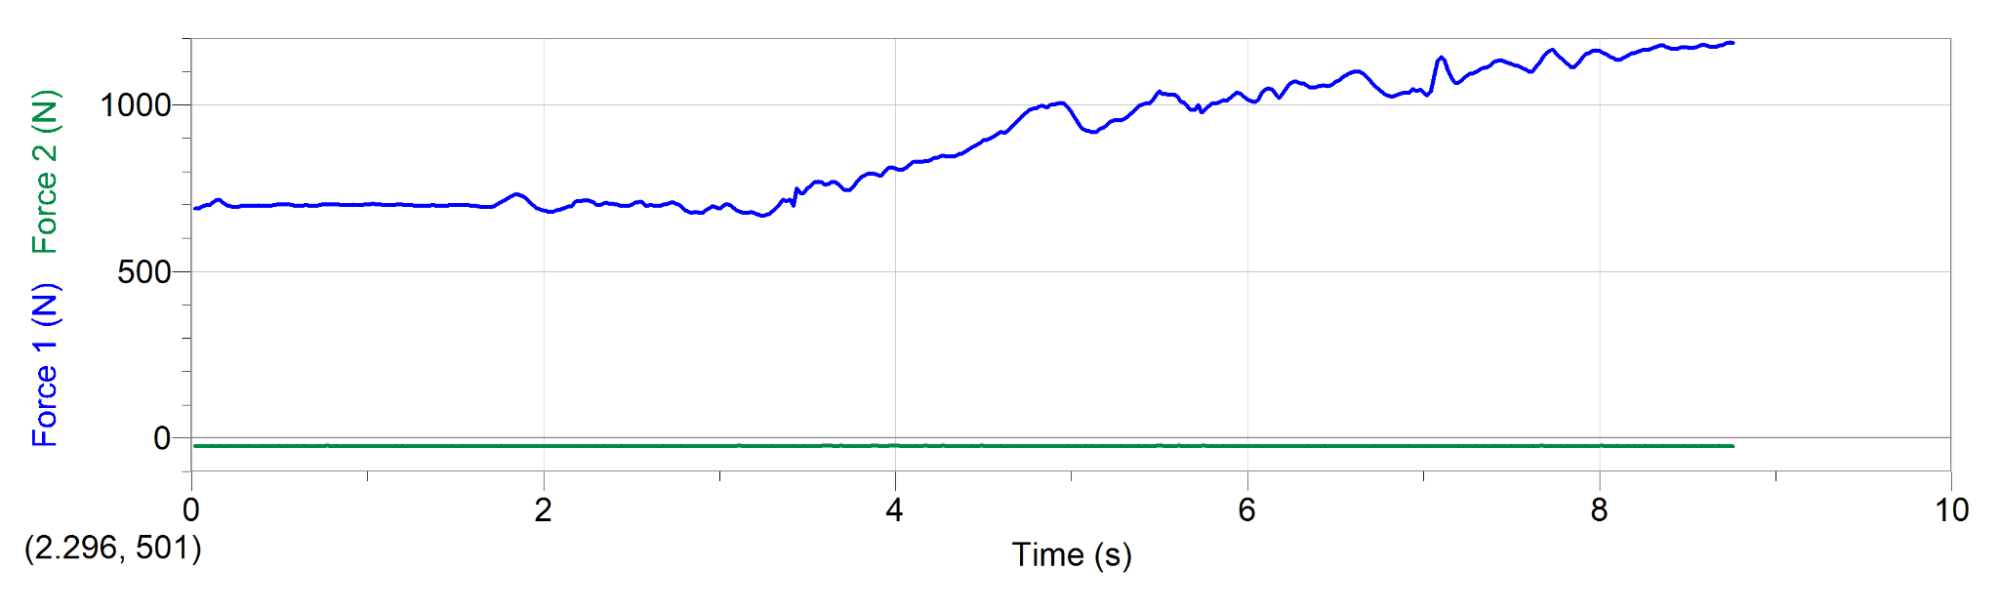
\includegraphics[width=\textwidth]{image12.png} 
        \end{mdframed}

        \paragraph*{17.}

        \begin{mdframed}
            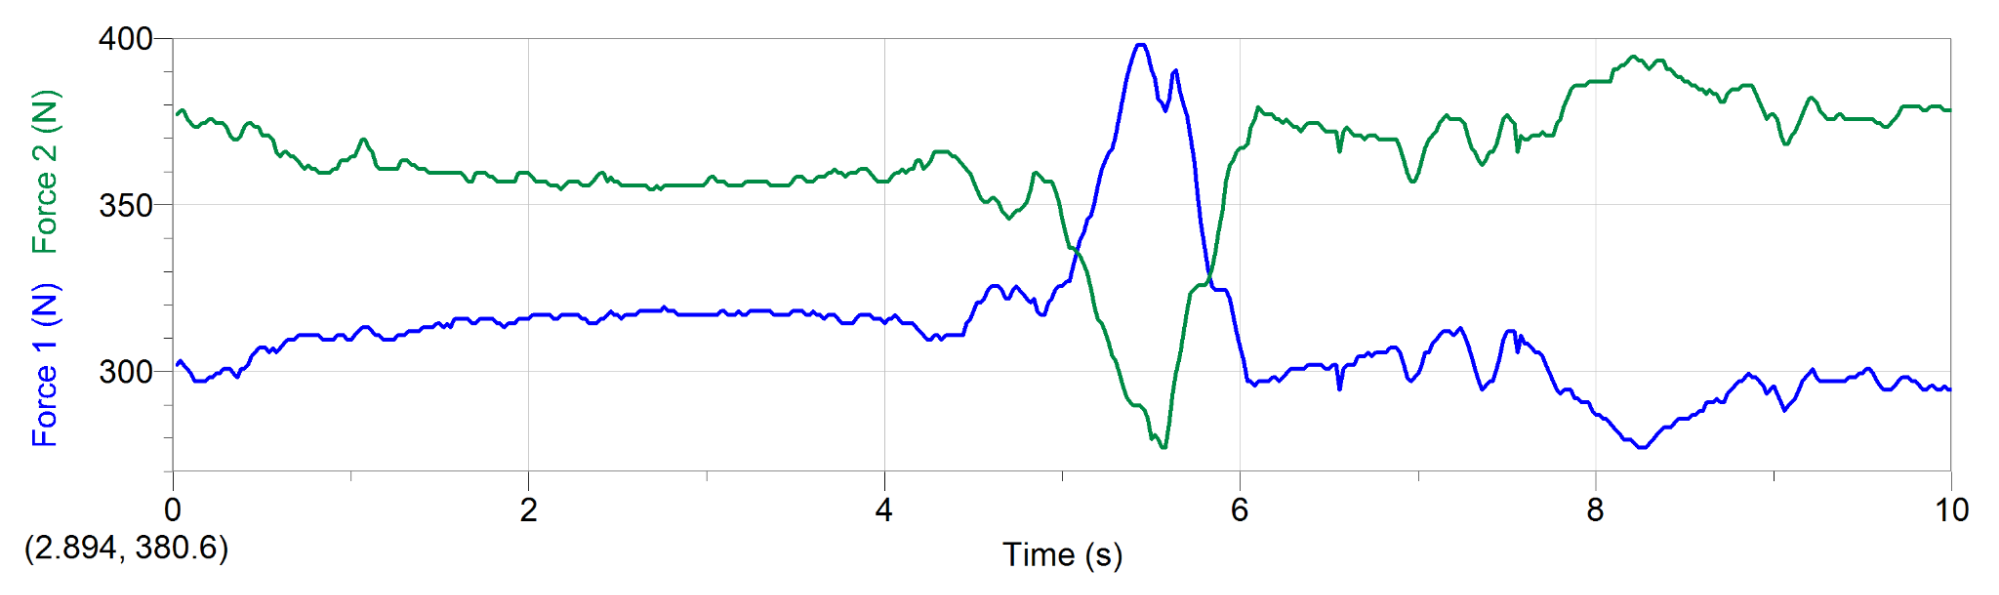
\includegraphics[width=\textwidth]{image17.png} 

            We had someone stand on the sensor, gave them a board, and then added a backpack on top of the board.
        \end{mdframed}

        \paragraph*{18.}

        \begin{mdframed}
            The more force used to jump, the higher you will go, which will take longer to accelerate you back down into the ground.
        \end{mdframed}

        \paragraph*{19.}

        \begin{mdframed}
            The wooden plank added to the weight.
        \end{mdframed}

        \paragraph*{20.}

        \begin{mdframed}
            Place the place upside down, press lightly on it, and then press harder.

            Put the plank back on with someone in the center, have one person step onto a side, and then another step onto the other side of the plank.
        \end{mdframed}

\end{document}